\section{Memoria de cálculo mecánica del prototipo manual}
\subsection{Entradas y trazabilidad}
Se leen los 1440 estados de
\texttt{serie\_M8x1.25\_h4mm.csv}, las auditorías geométricas del ensamble,
\texttt{Prototipo.stp} y \texttt{Matriz\_prototipo.stp}; no se ejecuta ni
modifica el acoplamiento 3C. EP2, páginas PDF10--11, define el árbol como
hilo corrido zincado de media pulgada y el inoxidable 304 para matriz y
rodillos. Ingeniería de Detalles, página PDF3, confirma accionamiento
manual y matriz 304; página PDF2 confirma carcasaABS. Los resultados antiguos
1,029\,kN y 3,255\,N\,m no se mezclan con el escenario vigente 918\,N/2,7804\,N\,m.
Los archivos anteriores se verifican por SHA256.

\subsection{Árbol: axial, torsión, flexión y rigidez}
Se reutiliza la metodología nominal de EP2 y 4B:
\begin{align}
 A&=\pi d^2/4,& I&=\pi d^4/64,& J&=\pi d^4/32,\\
 \sigma_N&=F/A,&\tau_T&=16T/(\pi d^3),&
 \sigma_{\rm VM}&=\sqrt{\sigma_N^2+3\tau_T^2},\\
 \delta_N&=FL/(EA),& \theta_T&=TL/(GJ),&G&=E/[2(1+\nu)].
\end{align}
Se usa la sección exterior nominal 12,7\,mm y longitud completa 200\,mm como
referencia de acortamiento/giro. El par se introduce en la unión del brazo
a 42,009\,mm por debajo de la guía inferior; la mano está 62\,mm más abajo.
La fuerza de mano se traslada a esa unión como fuerza más un par flector,
sin prolongar ficticiamente el árbol hasta la empuñadura.

Las guías ideales se sitúan en los centros de las placasCAD1 y 9,
separadas 75,991\,mm. Para la mano, el voladizo equivalente respecto de la
guía inferior es 104,009\,mm. El equilibrio produce reacciones radiales de
39,915\,N en la guía inferior y 23,064\,N en sentido contrario en la superior
para el máximo torque; no son cargas axiales ni reacciones de rodamientos
reales seleccionados. El momento manual máximo es 1,7526\,N\,m.
Se suma, como envolvente de orientaciones posibles en cada mismo estado,
el momento normal de compactación y el efecto de su resultante tangencial
desequilibrada. La máxima demanda nominal equivalente es 20,31\,MPa.

La flecha de 0,0183\,mm proviene de la formulación Euler--Bernoulli de EP2,
con ambos desplazamientos radiales restringidos en las guías, giros libres,
y superposición de fuerzas y pares correlacionados. El acero se modela
con $E=210$ GPa y $\nu=0,30$ como referencias elásticas, sin convertirlas
en una clase resistente. El modelo ideal de guía no equivale al contacto
real de un hilo corrido dentro de un taladro.
Como cribado de estabilidad, para 200\,mm y longitud eficaz conservadora
$KL=400$ mm resulta $P_{cr}=\pi^2EI/(KL)^2=16,54$ kN sobre la sección lisa.
No es un factor de seguridad de pandeo de la varilla roscada.

Los requisitos mínimos nominales quedan explícitos:
$S_y\geq20,31$ MPa para $n_y\geq1$ en la envolvente calculada;
para un material conocido, $n_y=S_y/\sigma_{\rm VM}$ se evaluará con
el diámetro resistente real y geometría de la unión. El zincado no define
$S_y$. No se trasladan al árbol los 640\,MPa candidatos del eje transversal.

El apoyo axial debe cerrar el camino matriz--árbol--bastidor o proporcionar
un camino alternativo explícito. La fuerza máxima de compactación es 918\,N;
los pesos de referencia de matriz 304 y árbol de acero suman 5,92\,N, de donde
se obtiene una demanda aproximada 924\,N. Los 608 de rodillos no constituyen
el apoyo axial del árbol 12,7\,mm. Las tuercas M12 nombradas en CAD no son
equivalentes a las de media pulgada documentadas en compras; comprobar
paso real de las tuercas de media pulgada, sin tratar M12 como pieza seleccionada.

\subsection{Rodamientos 608: cargas y capacidades}
Se importan las cuatro reacciones normales del 3C; no se reparten 918\,N en
cuatro partes iguales. Se añade el peso de cada rodillo,4,143\,N con densidad
de referencia 7900\,kg/m$^3$, repartido según sus centrosCAD. En cada rodamiento:
\begin{align}
 F_r(t)&=\sqrt{[R_N(t)-R_W]^2+[0,1R_N(t)]^2},\\
 P(t)&=1,2F_r(t),&P_0(t)&=F_r(t),\\
 P_{eq}&=\left[\frac 1{1440}\sum P(t)^3\right]^{1/3},&
 L_{10}&=(C/P_{eq})^3,&S_0&=C_0/\max(P_0).
\end{align}
La ponderación es por ángulo/revoluciones, no una velocidad manual
constante supuesta. Se adopta $F_a=0$ en la dirección del eje del rodillo;
la fuerza normal de compactación es radial para estos rodamientos.
El factor 1,2 corresponde al anillo exterior giratorio respecto de la carga
según el procedimiento publicado por NHBB\cite{nhbb_vida_exterior_2026},
como estimación conservadora de referencia, no una atribución de fórmula
particular a EZO. Se emplean las capacidades oficiales EZO 608ZZ
\cite{ezo_608zz_2026}; la marca de las unidades extraídas de ruedas sigue
sin identificar.
\begin{center}\begin{tabular}{rrrrr}\toprule
ID&$F_{r,\max}$[N]&$P_{eq}$[N]&$S_0$&$L_{10}$[$10^6$rev]\\\midrule
33 & 272,47 & 306,07 & 5,028 & 1253,4 \\
34 & 214,21 & 232,11 & 6,396 & 2873,9 \\
35 & 272,26 & 304,83 & 5,032 & 1268,7 \\
36 & 216,63 & 234,70 & 6,324 & 2779,9 \\
\bottomrule\end{tabular}\end{center}
La conversión a revoluciones de manivela usa rodadura ideal al radio
central del rodillo; no se publica vida en horas ni vida real de servicio
sin velocidad, lubricación, contaminación y montaje definidos.
Las capacidades de referencia no resuelven el alojamiento 24/22:
sin adaptador/asiento, la pista exterior no transmite correctamente
la reacción ni mantiene la holgura de operación.

\subsection{Matriz: apoyo y necesidad de FEM}
La placa perforada de 10\,mm incluye ligamentos mínimos 1,36\,mm y una transición
toroidal al cubo; no se sustituye por un disco macizo uniforme de 26\,mm.
La cara de arandela inferior realmente plana es el anillo 6,5--11,5\,mm,
área 282,743\,mm$^2$; el filete exterior limita el contacto plano antes de
alcanzar el radio 12\,mm de la arandela. Con $I_a=\pi(r_o^4-r_i^4)/4$:
\begin{equation}
 p_{\min,\max}=\frac{F}{\pi(r_o^2-r_i^2)}\mp\frac{Mr_o}{I_a}.
\end{equation}
Para los 1440 estados, $p_{\min}\geq3,054$ MPa y $p_{\max}\leq3,320$ MPa.
La excentricidad máxima 0,09195\,mm es menor que el núcleo central 3,7935\,mm.
Este equilibrio justifica un apoyo comprimido, pero no calcula la flexión
local de los ligamentos; por eso se ejecuta un FEM acotado, siguiendo la
elasticidad 3D de EP2, con geometría propia del prototipo.

\subsection{FEM ejecutado y comprobaciones numéricas}
Se importó el sólido de \texttt{Matriz\_prototipo.stp} con OpenCASCADE de
Gmsh 4.15.2, incluyendo 102 agujeros, cubo, toros y filetes existentes.
Se ensamblaron tetraedros lineales de elasticidad isotrópica con
scikit-fem 12.0.2, gradiente y tensor de tensiones por elemento; solución
CG con precondicionador de elasticidad PyAMG5.4.1, residuo relativo objetivo
$10^{-9}$. Las unidades son N,mm,MPa. Se adoptan $E=200000$ MPa,
$\nu=0,30$ y $R_{p0,2}=210$ MPa para 304 de referencia: $E$ y resistencia
se respaldan en Outokumpu H/P\cite{outokumpu_core_2026}; $\nu$ es hipótesis
elástica del modelo, no propiedad certificada del producto.

\textbf{Condición de borde:} desplazamientos nulos en la cara plana del
anillo de arandela en $y_{CAD}=26$ mm. Representa un apoyo rígido y adherente
con torque transmitido por la unión; no se supone que la matriz esté
soldada a toda la carcasa ni se restringe su periferia. El soporte axial
y el apriete que evitan deslizamiento deben materializarse; no fueron
modelados la tuerca, contacto con fricción ni el ABS. La suma de reacciones
axiales en sentido de tracción en la malla fina alcanza 0,195\,N.
Es diagnóstico de la fijación bilateral idealizada: debe existir retención
o precompresión, y no se interpreta esa suma como fuerza definitiva de una
tuerca. La presión global media positiva no demuestra por sí sola que
todo punto de contacto unilateral permanezca cerrado.

\textbf{Cargas:} se recuperaron las áreas por canal mediante las holguras
y pendientes ya guardadas, sin iterar ni actualizar 3C. El total de fuerzas
y el torque se contrastaron con el estado original. Se distribuyeron
tracciones axiales y tangenciales equivalentes sobre las paredes reales
de los canales, con reparto uniforme a lo largo de su longitud como
idealización; no se aplica presión a nodos inexistentes dentro de agujeros.
Esta idealización de tracciones no reproduce un campo local de presión
radial ni el comportamiento de biomasa dentro del canal.

Se detectó una inconsistencia del centroide tangencial de intersecciones
parciales del legado: algunos centroides individuales quedan fuera del
círculo de 3\,mm. En el estado 476, por ejemplo, el canal 12 tiene 3,898\,N y
distancia 9,024\,mm entre su centro y el centroide calculado. El código de
integración del primer momento tangencial incluye contribuciones de
intervalos verticales vacíos; el área y el primer momento radial usan
altura recortada. \textbf{No se corrigió ni reejecutó el 3C histórico.}
En el FEM se conserva cada fuerza de canal y el primer momento global
del estado, usando distribuciones positivas sobre las paredes con un
pequeño desplazamiento común de los centroides equivalentes. No se
interpretan los centroides parciales imposibles como puntos físicos.
La tabla de cargas de cada malla deja trazabilidad de esta regularización.
La presión de Holm y las fuerzas/torques importados no se sustituyen.

Se estudiaron los estados críticos correlacionados 476,541 y 625
(máximos de fuerza/torque, fuerza de rodillo y momento de normales).
No se combinaron máximos de estados diferentes ni se ejecutó un FEM de
los 1440 estados. Los resultados resistentes se circunscriben a estos
casos representativos. La convergencia se evalúa sobre la envolvente
máxima de esos mismos casos, con tolerancias declaradas 5\% para tensión
y 5\% para desplazamiento entre las dos últimas mallas.
\begin{center}\begin{tabular}{rrrr}\toprule
$h$[mm]&Tetraedros&$\max\sigma_{VM}$[MPa]&$\max|u|$[mm]\\\midrule
3,0 & 160305 & 31,849 & 0,01180 \\
2,3 & 284317 & 31,344 & 0,01230 \\
1,7 & 668262 & 35,918 & 0,01305 \\
1,25 & 1599263 & 36,375 & 0,01358 \\
\bottomrule\end{tabular}\end{center}
Cambios de las dos últimas mallas: tensión 1,27\% y
desplazamiento 4,05\%. La matriz cumple el cribado elástico bajo estas hipótesis, con $n_y=5,77$ respecto del límite de fluencia de referencia.
La convergencia de la solución discreta no valida automáticamente
la fricción, el apriete o la representación local de cargas de biomasa.
La tabla \texttt{convergencia\_por\_caso.csv} registra también los cambios
de cada caso individual: la convergencia de la envolvente no implica que
cada pico secundario haya alcanzado el mismo 5\%. El factor publicado
se refiere a la envolvente calculada, no a una cota matemática de todos
los estados angulares ni a una certificación de tensiones locales reales.
\begin{center}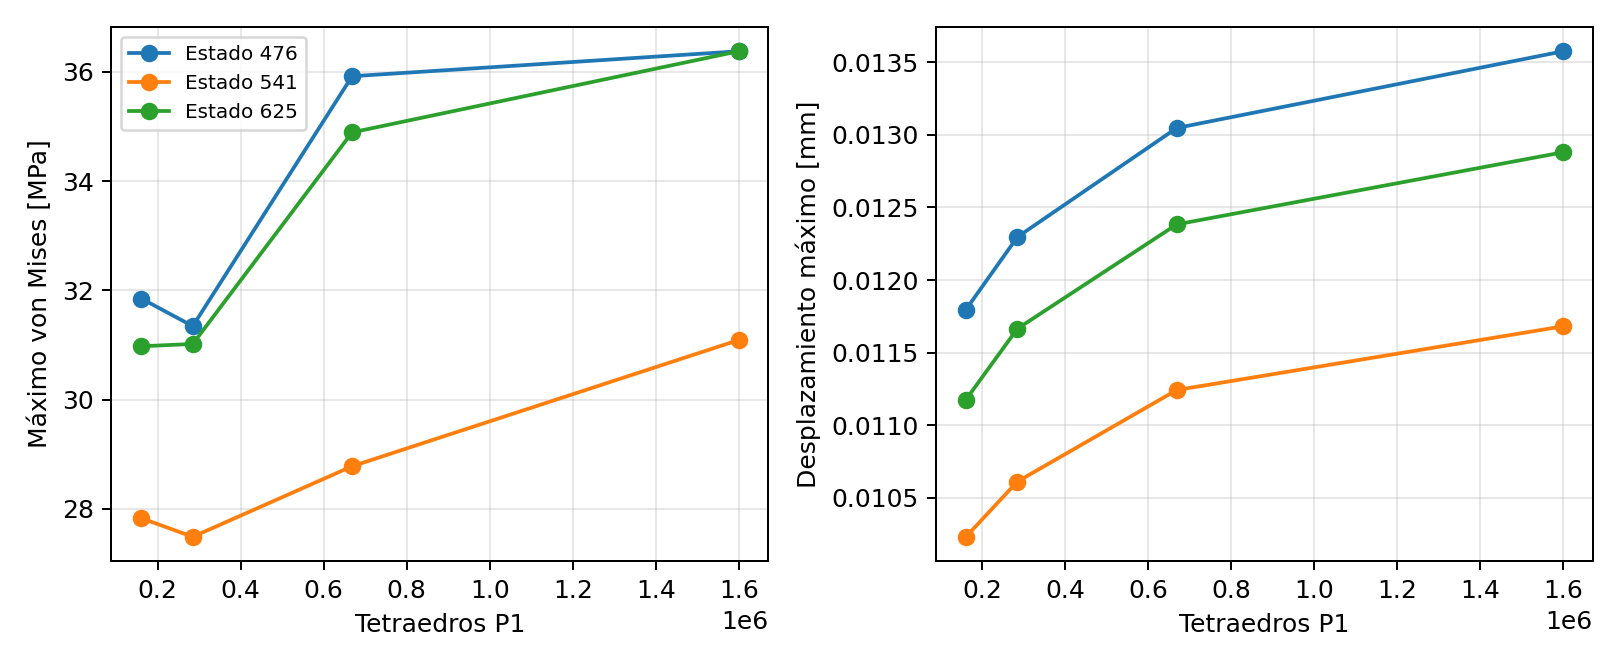
\includegraphics[width=.95\linewidth]{convergencia_matriz.png}\end{center}
\begin{center}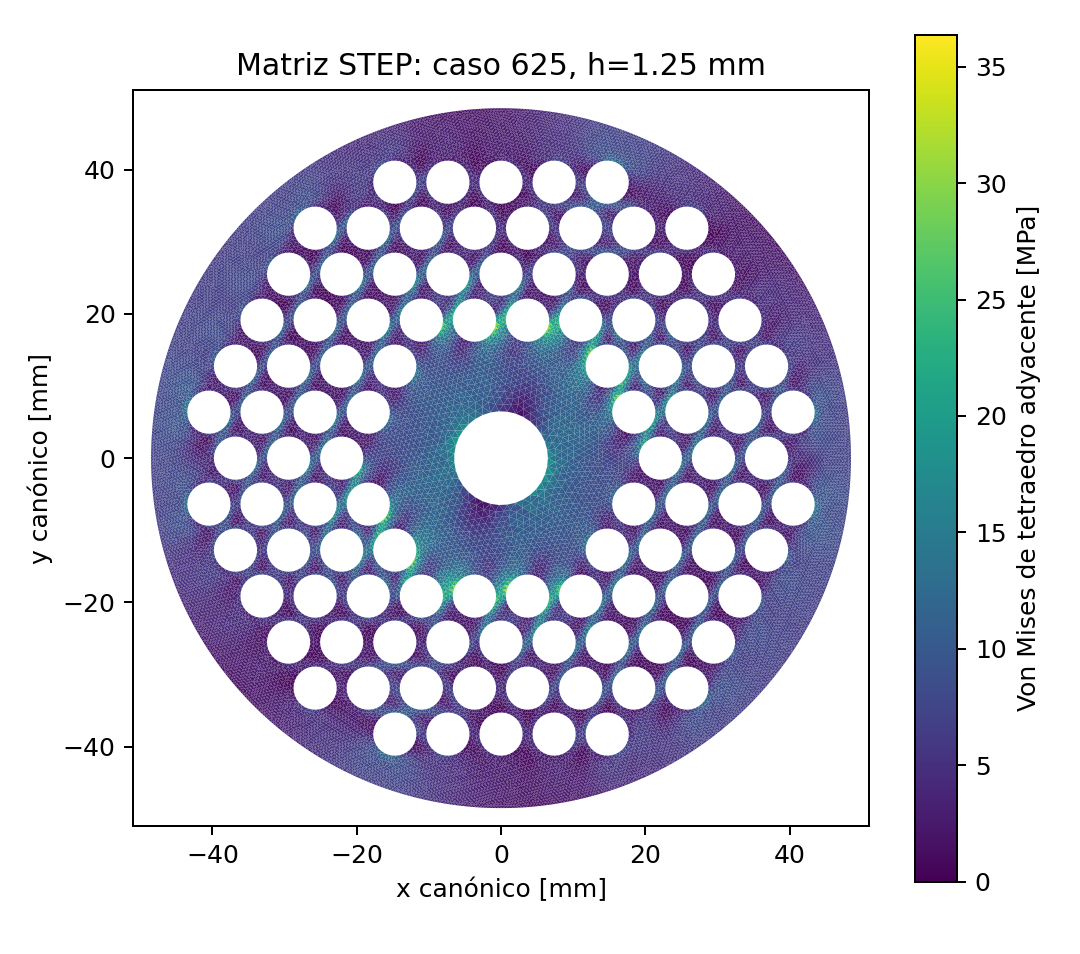
\includegraphics[width=.70\linewidth]{FEM_matriz_cara_trabajo.png}\end{center}
El mapa muestra el valor del tetraedro adyacente a cada triángulo de la
cara de trabajo, sin alisado nodal. El peso propio de la matriz,3,97\,N,
se omite en el FEM frente a 918\,N de compactación; se incluye como demanda
adicional del apoyo axial. La deformación de matriz no se realimenta
al 3C histórico en esta revisión.

\subsection{Manivela, pérdidas y uniones}
Se verifica el equilibrio $F_h=T/r_h$ para $r_h=0,165$m.
El máximo ideal 16,851\,N corresponde a aproximadamente 1,72\,kgf, sin convertir
ese valor en una recomendación ergonómica. Para pérdidas se publica
$F_h=T/(\eta r_h)$ con $\eta$ explícitamente hipotética, o de forma
general $F_h=(T+T_{\rm pérdidas})/r_h$. Sin pérdidas medidas no se declara
una fuerza real de accionamiento. Los atascos no se limitan por el
torque nominal calculado; faltan carga máxima manual admisible y capacidad
de las uniones para verificar esa condición.

En el tramo recto circular 15\,mm se estima
$\sigma_b=32T/(\pi d^3)=8,391$ MPa. El valor no describe el máximo en
agujero de unión, cambios de sección o codos. La fuerza tangencial
equivalente sobre la interfaz 12,7\,mm es $2T/d=437,86$ N. Falta el material
del brazo y la forma de transmitir el torque al árbol; no basta declarar
coincidencia de diámetros de agujero y eje.

Para la matriz--árbol por fricción, el radio de referencia de contacto
uniforme es $r_m=\frac23(r_o^3-r_i^3)/(r_o^2-r_i^2)=9,2315$ mm.
Una condición necesaria global es
\begin{equation}
 \mu r_m\sum N_i\geq 2,7804\,{\rm N\,m},\qquad
 \mu\sum N_i\geq 301,19\,{\rm N}.
\end{equation}
Se deben considerar las caras realmente comprimidas. No se asigna
coeficiente de fricción ni precarga arbitraria. Una unión positiva
alternativa requeriría su propia geometría y resistencia, no seleccionada
en esta entrega. Un apoyo axial deslizante también introduce pérdidas;
especificar su superficie o elemento rodante antes de dar por operativo
el conjunto.

\subsection{Cierre proporcionado al objetivo funcional}
Los datos indispensables se limitan a: grado/paso del árbol; material y
unión de manivela; asiento y retención de 608; apoyo axial del árbol y
apriete/retención de matriz. No se exige certificación industrial ni se
abre una comparación de nuevos motores, materiales o diámetros del M8.
La demanda es numéricamente compatible con accionamiento manual, pero no
demuestra extrusión estable ni montaje funcional sin resolver esas
interfaces. Los modelos y fuentes originales quedan intactos.
